\documentclass[11pt,letterpaper]{article}

% Import shared preamble relative to micro/chapters/
% ==============================================================================
% Shared Preamble: Principles of Economics Modular Curriculum
% Core Colors: SlateBlue (#1E293B) & Terracotta (#C2410C)
% ==============================================================================

\usepackage[utf8]{inputenc}
\usepackage[T1]{fontenc}
\usepackage{lmodern}
\usepackage[margin=1in]{geometry}
\usepackage{amsmath,amssymb,amsfonts,amsthm}
\usepackage{booktabs}
\usepackage{microtype}
\usepackage{enumitem}
\usepackage{fancyhdr}
\usepackage{titlesec}
\usepackage{xcolor}
\usepackage{tikz}
\usepackage{pgfplots}
\usepackage{mdframed}
\usepackage[hidelinks,colorlinks=true,linkcolor=SlateBlue,citecolor=SlateBlue,urlcolor=Terracotta]{hyperref}

\pgfplotsset{compat=1.18}
\usetikzlibrary{arrows.meta,positioning,calc,patterns,decorations.pathreplacing}

% --- Color Palette Definitions ---
\definecolor{SlateBlue}{HTML}{1E293B}      % Primary Accent / Structure
\definecolor{Terracotta}{HTML}{C2410C}     % Secondary Accent / Emphasis
\definecolor{ForestGreen}{HTML}{15803D}    % Equilibrium / Positive Shocks
\definecolor{LightSlate}{HTML}{F8FAFC}     % Box Background Fill
\definecolor{BorderGray}{HTML}{CBD5E1}     % Neutral Borders
\definecolor{LightTerracotta}{HTML}{FFF7ED}% Cautionary / Principle Fill

% --- Section Heading Styling ---
\titleformat{\section}
  {\normalfont\Large\bfseries\color{SlateBlue}}{\thesection}{1em}{}[\titlerule]
\titleformat{\subsection}
  {\normalfont\large\bfseries\color{SlateBlue}}{\thesubsection}{1em}{}
\titleformat{\subsubsection}
  {\normalfont\normalsize\bfseries\color{Terracotta}}{\thesubsubsection}{1em}{}

% --- Header and Footer Configuration ---
\pagestyle{fancy}
\fancyhf{}
\renewcommand{\headrulewidth}{0.4pt}
\renewcommand{\footrulewidth}{0.4pt}
\fancyhead[L]{\small\scshape\color{SlateBlue}\leftmark}
\fancyhead[R]{\small\color{SlateBlue}Principles of Economics}
\fancyfoot[C]{\thepage}

% --- Custom Environments (mdframed) ---

% 1. Core Principle Box
\newmdenv[
  linecolor=Terracotta,
  linewidth=1.5pt,
  backgroundcolor=LightTerracotta,
  innertopmargin=10pt,
  innerbottommargin=10pt,
  innerrightmargin=12pt,
  innerleftmargin=12pt,
  roundcorner=4pt,
  skipabove=12pt,
  skipbelow=12pt
]{coreprinciple}

% 2. Empirical Case Study Box
\newmdenv[
  linecolor=SlateBlue,
  linewidth=1.5pt,
  backgroundcolor=LightSlate,
  innertopmargin=10pt,
  innerbottommargin=10pt,
  innerrightmargin=12pt,
  innerleftmargin=12pt,
  roundcorner=4pt,
  skipabove=12pt,
  skipbelow=12pt
]{casestudy}

% 3. Key Takeaways Box
\newmdenv[
  linecolor=BorderGray,
  linewidth=1pt,
  backgroundcolor=white,
  innertopmargin=10pt,
  innerbottommargin=10pt,
  innerrightmargin=12pt,
  innerleftmargin=12pt,
  roundcorner=4pt,
  skipabove=12pt,
  skipbelow=12pt
]{takeaways}

% Environment Title Helpers
\newcommand{\boxheader}[2]{{\noindent\bfseries\color{#1}\Large #2}\vspace{0.4em}\par}

\begin{document}

\title{\Huge\bfseries\color{SlateBlue} Chapter 1: Foundations of Microeconomic Analysis \& Core Principles}
\author{\large Principles of Microeconomics Curriculum}
\date{}
\maketitle

\thispagestyle{plain}

\begin{abstract}
This chapter establishes the axiomatic foundation of microeconomic theory, structured around the decisions of individual agents operating under scarcity. Aligned with the conceptual framework of Eric Chiang's \textit{Microeconomics: Principles for a Changing World}, we formalize opportunity cost, marginal decision rules, trade-offs, and behavioral responsiveness to incentives. Analytical formulations are paired with empirical evidence from contemporary social science literature, and marginal net benefit optimization is modeled via native vector graphics.
\end{abstract}

\tableofcontents
\vspace{1.5em}
\hrule
\vspace{1.5em}

% ==============================================================================
\section{The Core Economic Problem: Scarcity and Allocation}
% ==============================================================================

Economics is the formal study of how societies allocate scarce resources among competing, unlimited wants. A resource is categorized as \textbf{scarce} whenever the quantity demanded at a zero nominal price exceeds the total quantity available from nature.

\begin{coreprinciple}
\boxheader{Terracotta}{Core Axiom 1: Scarcity Enforces Trade-offs}
Because productive inputs (land, labor, physical capital, and entrepreneurial human capital) are strictly finite, every choice to produce or consume a good requires forfeiting the opportunity to produce or consume an alternative bundle. Society cannot achieve bliss points where all human wants are simultaneously satisfied.
\end{coreprinciple}

Formally, consider an allocation space defined over an economy with endowment vector $\boldsymbol{\omega} \in \mathbb{R}^K_+$. The feasibility set of consumption bundles $\mathbf{X}$ is constrained such that:
\begin{equation}
    \sum_{i=1}^N \mathbf{x}_i \le \boldsymbol{\omega}
\end{equation}
Any movement within the interior or along the frontier of this resource simplex necessitates an exchange of one utility-generating asset for another.

% ==============================================================================
\section{Opportunity Cost and the Trade-off Frontier}
% ==============================================================================

The true economic cost of any decision is not merely the monetary expense, but its \textbf{opportunity cost}: the subjective and objective valuation of the next-best alternative foregone.

\subsection{Accounting Cost vs. Economic Cost}
Standard accounting frameworks isolate explicit historical cash outlays:
\begin{equation}
    \text{Accounting Cost} = \sum \text{Explicit Outlays}
\end{equation}
Microeconomic analysis incorporates implicit costs, including the foregone return on alternative capital deployments and the opportunity cost of owner-allocated labor:
\begin{equation}
    \text{Economic Cost} = \text{Explicit Outlays} + \text{Implicit Opportunity Costs}
\end{equation}
Consequently, \textbf{Economic Profit} ($\pi_e$) diverges fundamentally from \textbf{Accounting Profit} ($\pi_a$):
\begin{equation}
    \pi_e = \text{Total Revenue} - (\text{Explicit Costs} + \text{Implicit Costs}) = \pi_a - \text{Implicit Costs}
\end{equation}
When $\pi_e = 0$, the decision-maker earns a \textit{normal rate of return}, precisely compensating them for their capital and time at market-clearing parity.

% ==============================================================================
\section{Rationality, Incentives, and Human Action}
% ==============================================================================

Microeconomic models rely on the behavioral assumption of purposeful rationality. An economic agent is defined as rational if their preference relation $\succeq$ satisfies two core properties:
\begin{enumerate}[label=(\alph*)]
    \item \textbf{Completeness:} $\forall\, x, y \in \mathbf{X}$, either $x \succeq y$, $y \succeq x$, or both ($x \sim y$).
    \item \textbf{Transitivity:} $\forall\, x, y, z \in \mathbf{X}$, if $x \succeq y$ and $y \succeq z$, then $x \succeq z$.
\end{enumerate}

Rational agents react predictably to changes in incentives. When the marginal penalty associated with an action increases, or the marginal reward diminishes, agents substitute away from that action.

\begin{casestudy}
\boxheader{SlateBlue}{Empirical Case Study: Unintended Incentive Distortions in Daycare Punctuality}
In a controlled field experiment across 10 day-care centers in Haifa, Israel, economists Uri Gneezy and Aldo Rustichini (2000) evaluated the introduction of a modest monetary fine levied on parents who arrived more than 10 minutes late to pick up their children.

\textbf{Empirical Observation:} Following the introduction of the fine, late pickups \textit{doubled} rather than decreased.

\textbf{Economic Explanation:} Prior to the fine, parents operated under a non-monetary social contract governed by guilt and civic norms. Introducing a small financial fine converted an ambiguous social taboo into a priced commodity. The fine was low enough that parents willingly paid it to purchase additional childcare time, and the social norm did not recover even after the fine was removed.
\end{casestudy}

% ==============================================================================
\section{Marginal Analysis: Optimization via Differential Calculus}
% ==============================================================================

Economic decisions are rarely binary (all-or-nothing); they occur at the margin. Optimal resource allocation requires comparing the incremental addition to total benefit with the incremental addition to total cost.

Let total benefit be represented by a twice-differentiable, strictly concave function $B(q)$ such that $B'(q) > 0$ and $B''(q) < 0$. Let total cost be represented by a twice-differentiable, strictly convex function $C(q)$ such that $C'(q) > 0$ and $C''(q) > 0$.

The agent's objective is to maximize Net Social or Private Benefit $N(q)$:
\begin{equation}
    \max_{q \ge 0} N(q) = B(q) - C(q)
\end{equation}

The first-order necessary condition (FONC) for an interior optimum requires:
\begin{equation}
    \frac{dN}{dq} = B'(q) - C'(q) = 0 \implies MB(q^*) = MC(q^*)
\end{equation}

The second-order sufficient condition (SOSC) confirms that $q^*$ achieves a strict global maximum:
\begin{equation}
    \frac{d^2N}{dq^2} = B''(q) - C''(q) < 0 \quad (\text{since } B''(q) < 0 \text{ and } C''(q) > 0)
\end{equation}

\subsection{Vector Representation of Marginal Net Benefit Optimization}

Figure~\ref{fig:marginal_optimization} illustrates the equilibrium quantity $q^*$ where $MB = MC$. At any output level $q_1 < q^*$, $MB > MC$, implying that expanding activity yields a positive net gain ($\Delta N > 0$). At $q_2 > q^*$, $MC > MB$, meaning total net benefit is eroded by excessive expansion.

\begin{figure}[htbp]
\centering
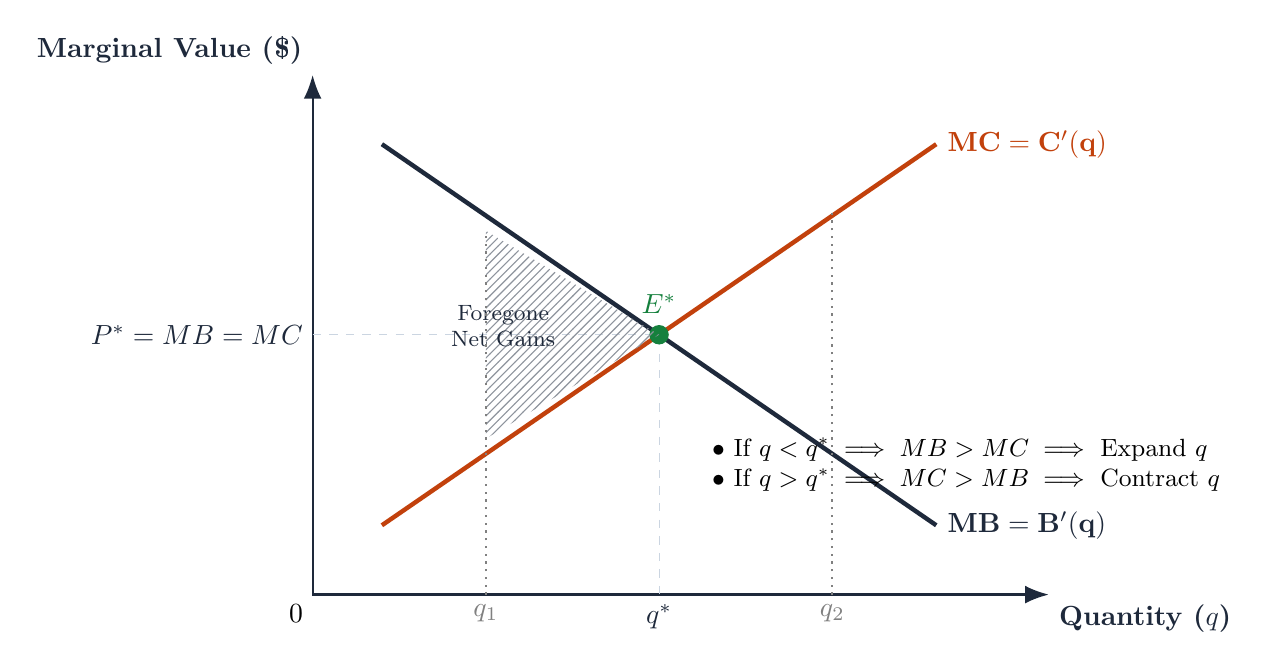
\begin{tikzpicture}[scale=1.1]
    % Coordinate axes
    \draw[{Latex[length=3mm]}-{Latex[length=3mm]}, thick, color=SlateBlue] (0,6) node[above left] {\bfseries Marginal Value (\$)} -- (0,0) -- (8.5,0) node[below right] {\bfseries Quantity ($q$)};
    
    % Origin label
    \node[below left] at (0,0) {$0$};

    % Grid lines (subtle)
    \draw[dashed, color=BorderGray] (0,3) -- (4,3) -- (4,0);

    % Curves
    % Marginal Benefit Curve (Downward sloping)
    \draw[ultra thick, color=SlateBlue] (0.8, 5.2) -- (7.2, 0.8) node[right] {$\mathbf{MB = B'(q)}$};
    
    % Marginal Cost Curve (Upward sloping)
    \draw[ultra thick, color=Terracotta] (0.8, 0.8) -- (7.2, 5.2) node[right] {$\mathbf{MC = C'(q)}$};

    % Equilibrium Intersection
    \filldraw[color=ForestGreen] (4,3) circle (3pt) node[above=4pt, font=\bfseries] {$E^*$};
    
    % Shaded deadweight loss / foregone gains if underproducing
    \fill[pattern=north east lines, pattern color=SlateBlue!50] (2, 4.2) -- (2, 1.8) -- (4, 3) -- cycle;
    \node[font=\footnotesize, color=SlateBlue, align=center] at (2.2, 3.1) {Foregone\\Net Gains};

    % Points on X and Y axes
    \node[below, font=\bfseries, color=SlateBlue] at (4,0) {$q^*$};
    \node[left, font=\bfseries, color=SlateBlue] at (0,3) {$P^* = MB = MC$};

    % Disequilibrium indicators
    \node[below, color=gray] at (2,0) {$q_1$};
    \node[below, color=gray] at (6,0) {$q_2$};
    
    \draw[dotted, thick, color=gray] (2,0) -- (2,4.2);
    \draw[dotted, thick, color=gray] (6,0) -- (6,4.4);
    
    % Annotations
    \node[font=\small, align=left, anchor=west] at (4.5, 1.5) {
        $\bullet$ If $q < q^* \implies MB > MC \implies$ Expand $q$\\
        $\bullet$ If $q > q^* \implies MC > MB \implies$ Contract $q$
    };
\end{tikzpicture}
\caption{The Equimarginal Decision Rule: Maximum net benefit occurs exclusively at the intersection of Marginal Benefit ($MB$) and Marginal Cost ($MC$).}
\label{fig:marginal_optimization}
\end{figure}

% ==============================================================================
\section{Positive vs. Normative Analysis}
% ==============================================================================

Methodological clarity in microeconomic investigation requires an absolute separation between objective descriptive claims and value-laden prescriptive assertions:

\begin{itemize}
    \item \textbf{Positive Economics:} Examines testable hypotheses regarding cause-and-effect relationships. Formulated in conditional terms (``If policy $A$ is enacted, then variable $Y$ will change by $\Delta Y$''). These assertions are falsifiable using econometric observation.
    \item \textbf{Normative Economics:} Evaluates policies through ethical frameworks, social welfare judgments, or ideological priorities (``The government \textit{ought} to reduce income inequality through wealth redistribution''). These claims cannot be settled by empirical testing alone.
\end{itemize}

\begin{table}[htbp]
\centering
\caption{Comparative Structure of Economic Statements}
\label{tab:positive_normative}
\begin{tabular}{@{}lll@{}}
\toprule
\textbf{Attribute} & \textbf{Positive Analysis} & \textbf{Normative Analysis} \\ \midrule
\textbf{Underlying Question} & What is, or what will occur? & What ought to be? \\
\textbf{Epistemic Status}    & Falsifiable via empirical data & Non-falsifiable ethical preference \\
\textbf{Role in Policy}     & Forecasts deadweight loss, prices & Defines equity criteria, goals \\
\textbf{Standard Example}    & Rent control reduces housing supply & Rent control should be implemented \\ \bottomrule
\end{tabular}
\end{table}

% ==============================================================================
\section{Efficiency vs. Equity: The Core Policy Trade-Off}
% ==============================================================================

Public policy constantly balances allocative efficiency against distributional equity:
\begin{itemize}
    \item \textbf{Pareto Efficiency:} An allocation of resources where it is impossible to make any one individual better off without making at least one individual worse off.
    \item \textbf{Distributional Equity:} The perceived fairness or justice in the dispersion of economic output across members of society.
\end{itemize}

Policies designed to compress income dispersion (e.g., progressive income taxation, statutory minimum wages) frequently introduce price distortions that generate deadweight losses, trading off total societal wealth to achieve greater distributional parity.

% ==============================================================================
\section{Empirical Literature: Sunk Cost Fallacy}
% ==============================================================================

Standard microeconomic optimization dictates that rational forward-looking decisions should ignore \textbf{sunk costs}—expenditures already incurred that cannot be recovered. Because sunk costs are fixed across all future states of the world, their marginal cost is zero ($MC_{\text{sunk}} = 0$).

\begin{casestudy}
\boxheader{SlateBlue}{Empirical Case Study: The Behavioral Sunk Cost Effect}
Hal Arkes and Catherine Blumer (1985) executed a field experiment evaluating whether sunk costs systematically bias real-world human behavior. 

\textbf{Experimental Setup:} Patrons purchasing season tickets to a university theatre series were randomly assigned to three groups:
\begin{enumerate}
    \item Paid standard full retail price (\$15).
    \item Received an unexpected \$2 discount per ticket (\$13).
    \item Received an unexpected \$7 discount per ticket (\$8).
\end{enumerate}

\textbf{Findings:} During the first half of the season, patrons who paid the full retail price attended significantly more plays than patrons who received the blind discounts. Because the physical seats and production quality were identical across all cohorts, traditional neoclassical theory predicted identical attendance rates. The observed divergence demonstrated that individuals systematically commit resources to justify prior unrecoverable investments.
\end{casestudy}

% ==============================================================================
\section{Key Takeaways \& Problem Set}
% ==============================================================================

\begin{takeaways}
\boxheader{SlateBlue}{Summary of Foundational Concepts}
\begin{enumerate}
    \item \textbf{Scarcity} requires allocation mechanisms; prices act as signals to coordinate decentralized preferences.
    \item \textbf{Opportunity cost} measures the value of the most desirable foregone alternative, combining explicit accounting expenses and implicit opportunity costs.
    \item \textbf{Optimization at the Margin:} A rational decision-maker maximizes net welfare by continuing an activity up to the exact point where $MB(q^*) = MC(q^*)$. Sunk costs must be fully disregarded.
    \item \textbf{Positive vs. Normative:} Positive analysis models testable empirical facts; normative analysis debates value-based objectives.
\end{enumerate}
\end{takeaways}

\subsection{Analytical Discussion Problems}
\begin{enumerate}
    \item An economics student spends 3 hours studying for an exam, scoring an 88\%. If they had not studied, they would have scored a 60\% and worked at their part-time job earning \$16 per hour. Calculate the explicit financial cost and the implicit opportunity cost of the study session.
    \item Suppose the marginal benefit of adding a municipal transit route is $MB(q) = 120 - 4q$ and the marginal cost is $MC(q) = 20 + 6q$, where $q$ is the number of routes. 
    \begin{enumerate}[label=(\alph*)]
        \item Calculate the socially optimal number of transit routes $q^*$.
        \item Determine the total net social benefit gained at this optimum relative to $q = 0$.
    \end{enumerate}
    \item Evaluate the following statement: \textit{``The state should subsidize public higher education because an educated populace improves civic participation.''} Categorize each clause as positive or normative economics.
\end{enumerate}

\end{document}